\documentclass[%
 aip,
% jmp,
% bmf,
% sd,
% rsi,
 amsmath,amssymb,
%preprint,%
 reprint,%
%author-year,%
%author-numerical,%
% Conference Proceedings
]{revtex4-1}

\usepackage{graphicx}% Include figure files
\usepackage{dcolumn}% Align table columns on decimal point
\usepackage{bm}% bold math
%\usepackage[mathlines]{lineno}% Enable numbering of text and display math
%\linenumbers\relax % Commence numbering lines

\usepackage[utf8]{inputenc}
\usepackage[T1]{fontenc}
\usepackage{mathptmx}
\usepackage{etoolbox}
\usepackage{hyperref}
\usepackage{svg}

%% Apr 2021: AIP requests that the corresponding 
%% email to be moved after the affiliations
\makeatletter
\def\@email#1#2{%
 \endgroup
 \patchcmd{\titleblock@produce}
  {\frontmatter@RRAPformat}
  {\frontmatter@RRAPformat{\produce@RRAP{*#1\href{mailto:#2}{#2}}}\frontmatter@RRAPformat}
  {}{}
}%
\makeatother
\begin{document}

\preprint{AIP/123-QED}

\title[Sample title]{Sample Title:\\with Forced Linebreak}
% Force line breaks with \\
\author{A. Author}
 \altaffiliation[Also at ]{Physics Department, XYZ University.}%Lines break automatically or can be forced with \\
\author{B. Author}%
 \email{Second.Author@institution.edu.}
\affiliation{ 
Authors' institution and/or address%\\This line break forced with \textbackslash\textbackslash
}%

\author{C. Author}
 \homepage{http://www.Second.institution.edu/~Charlie.Author.}
\affiliation{%
Second institution and/or address%\\This line break forced% with \\
}%

\date{\today}% It is always \today, today,
             %  but any date may be explicitly specified

\begin{abstract}
    An article usually includes an abstract, a concise summary of the work
    covered at length in the main body of the article. It is used for
    secondary publications and for information retrieval purposes. 
\end{abstract}

\maketitle

\begin{quotation}
    The ``lead paragraph'' is encapsulated with the \LaTeX\
    %
    The lead paragraph will only be found in an article being prepared for the journal \textit{Chaos}.
\end{quotation}

\section{\label{sec:level1}INTRODUCTION\protect\\ }
% The line break was forced \lowercase{via} \textbackslash\textbackslash
The color of the background represents the order parameter $r$ of the system. The color of the snapshots represents the phase of the oscillators. The color of the arrows represents the direction of the velocity of the oscillators. The size of the arrows represents the speed of the oscillators. 

\section{model}
Oscillators have a spatial position $\mathbf{r}_i=\left( x_i, y_i \right) $ and an internal phase $\theta_i$ which evoleve according to equations:

\begin{eqnarray}
    \dot{x}_i&=&v\cos \theta _i\;,\label{eq:dotxi}
  \\
    \dot{y}_i&=&v\sin \theta _i\;,\label{eq:dotyi}
  \\
    \dot{\theta}_i&=&\omega _i+\lambda \sum_{j=1}^N{A_{ij}\sin \left( \theta _j-\theta _i \right)}
    \label{eq:dotthetai}
\end{eqnarray}
for $i=1,2,\ldots,N$, where $N$ is the number of oscillators. As per Eq.~(\ref{eq:dotxi}) and (\ref{eq:dotyi}), each oscillator moves with a constant speed $v$ in the direction of its current phase $\theta_i$. The phase $\theta_i$ evolves according to Eq.~(\ref{eq:dotthetai}), where $\omega_i$ is the natural frequency of the $i$th oscillator, $\lambda$ is the coupling strength, and $A$ is the adjacency matrix of the network, with $A_{ij}=1$ if there is a connection from $i$th to $j$th oscillator, and $A_{ij}=0$ otherwise. We can consider Eq.~(\ref{eq:dotxi})-(\ref{eq:dotthetai}) as a generalization of the Kuramoto model and the Vicsek model in the sense that it includes both the phase and the spatial position of the oscillators.

Each oscillator $i$ is connected to all the oscillators within a
action radius $d_0$ of its position. The adjacency matrix $A$ is defined as:

\begin{equation}
    A_{ij}=\begin{cases}
        1,&		\left| \mathbf{r}_i-\mathbf{r}_j \right|\le d_0\\
        0,&		\left| \mathbf{r}_i-\mathbf{r}_j \right|>d_0\\
    \end{cases}
\end{equation}
where $\left| \mathbf{r}_i-\mathbf{r}_j \right|$ is the Euclidean distance between the $i$th and $j$th oscillators. 

For simplicity, we consider oscillators are initially distributed uniformly in a two-dimensional square with side length $L$ and periodic boundary conditions. Their positions $\mathbf{r}_i\left( t \right) =\left( x_i\left( t \right) ,y_i\left( t \right) \right) $ at given time $t$ are given by:

\begin{equation}
    \begin{array}{c}
        x_i\left( t+\Delta t \right) =x_i\left( t \right) +v\cos \theta _i\left( t \right) \Delta t\,\,\mathrm{mod}\ L,\\
        x_i\left( t+\Delta t \right) =x_i\left( t \right) +v\cos \theta _i\left( t \right) \Delta t\,\,\mathrm{mod}\ L,\\
    \end{array}
\end{equation}
where $\Delta t$ is the discrete time step. When two oscillators are on opposite sides of the square, the absolute value of the difference between one of their coordinates is greater than $L/2$. In this case, we take the minimum distance between them, which is the distance between the two points in the periodic boundary conditions. For a given pair of points $\mathbf{r}_i$ and $\mathbf{r}_j$, the distance between them is $\left| \mathbf{r}_i-\bar{\mathbf{r}}_j \right|$, where $\bar{\mathbf{r}}_j=\left( \bar{x}_j,\bar{y}_j \right)$ is the adjusted position of the $j$th oscillator, given by:
\begin{eqnarray}
    \bar{x}_j=\begin{cases}
        x_j,&		\left| x_i-x_j \right|\le L/2\\
        x_j+L,&		x_i-x_j>L/2\\
        x_j-L,&		x_i-x_j>L/2\\
    \end{cases},
    \\
    \bar{y}_j=\begin{cases}
        y_j,&		\left| y_i-y_j \right|\le L/2\\
        y_j+L,&		y_i-y_j>L/2\\
        y_j-L,&		y_i-y_j>L/2\\
    \end{cases}.
\end{eqnarray}
$\left| \mathbf{r}_i-\bar{\mathbf{r}}_j \right|$ can be proved to be the minimum distance between $\mathbf{r}_i$ and $\mathbf{r}_j$ in the periodic boundary conditions (see the proof in Appendix \ref{sec:adj_pos}).

Finally, we consider that the natural frequencies $\omega_i$ are distributed in two symmetric uniform distributions. Exactly half of the oscillators have natural frequencies in the range $\left[ \omega _{\min},\omega _{\max} \right]$ ($\omega_i \sim U\left( \omega _{\min},\omega _{\max} \right), i=1,2,\ldots,N/2$) and the other half in the range $\left[ -\omega _{\max},-\omega _{\min} \right]$ ($\omega_i \sim U\left( -\omega _{\max},-\omega _{\min} \right), i=N/2+1,N/2+2,\ldots,N$).

\section{behavior}

\begin{figure*}
    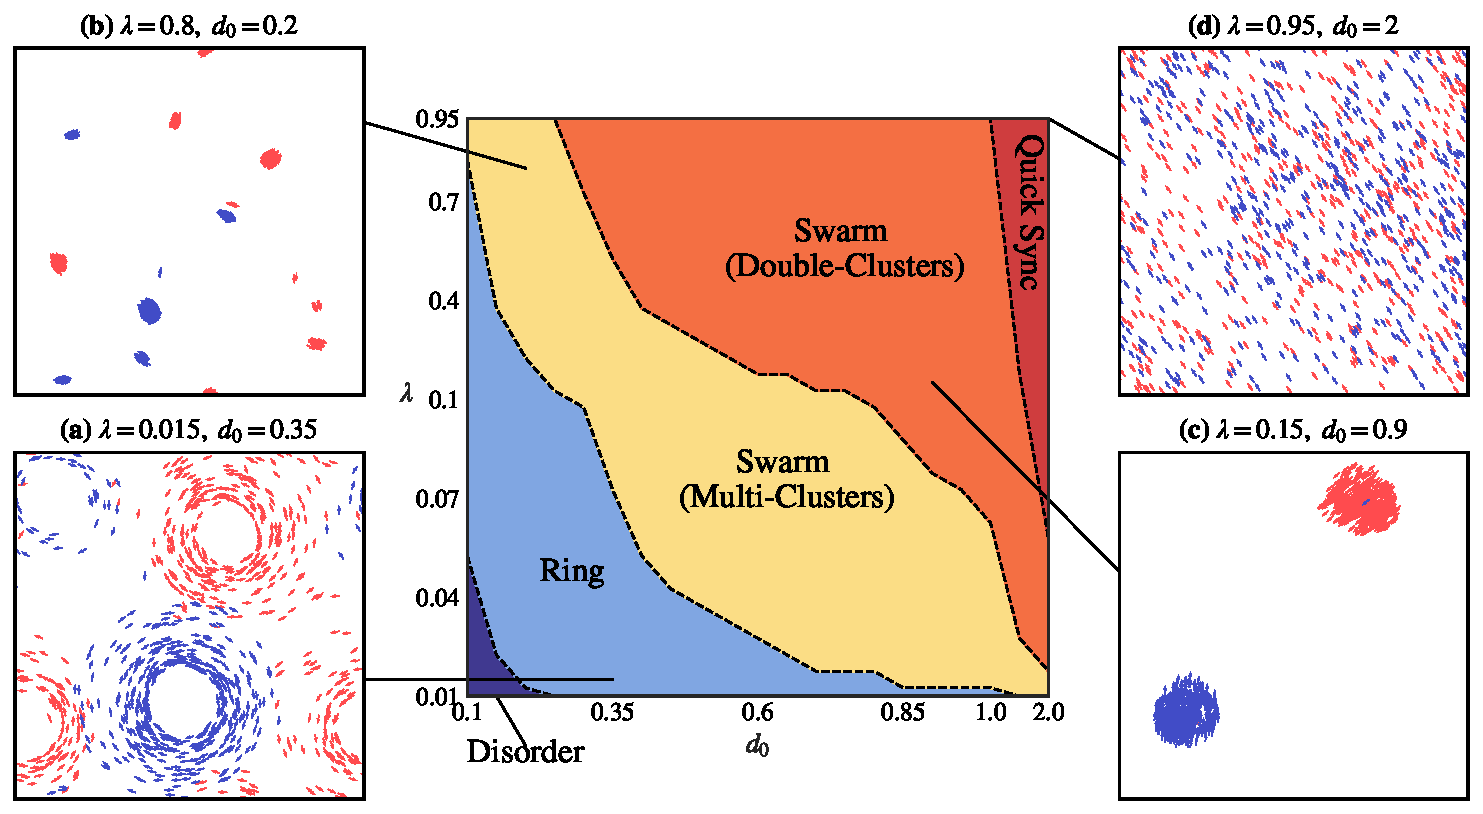
\includegraphics[width=\textwidth]{./figs/phaseDiagram.pdf}
    \caption{
        \label{fig:phaseDiagram} Phase diagram of model Eq.~(\ref{eq:dotxi})-(\ref{eq:dotthetai}) in the $(\lambda$-$d_0)$ plane. The boundary between the states is analytic approximations given by \textcolor{red}{XXXXXXX}. The snapshots of Ring ($\lambda=0.015,\ d_0=0.35$), Swarm (Multi-Clusters) ($\lambda=0.8,\ d_0=0.2$), Swarm (Double-Clusters) ($\lambda=0.15,\ d_0=0.9$) and Quick Sync ($\lambda=0.95,\ d_0=2$) states are shown around the diagram. For the sake of clarity, the scale of $\lambda$ and $d_0$ is non-linear (For $\lambda$ in $\left[ 0.01, 0.1 \right]$ and $\left[ 0.1, 1 \right]$, step length is $0.1$ and $0.05$, respectively. For $d_0$ in $\left[ 0.1, 1 \right]$ and $\left[ 1, 2 \right]$, step length is $0.05$ and $0.5$, respectively). Other parameters are $N=1000$, $v=3$, $L=10$, $\omega _{\min}=1$, $\omega _{\max}=3$.
    }
\end{figure*}

We performed numerical simulations of the model to probe the behavior of its solutions (see Appendix \ref{sec:numerics} for details on the numerical methods). 
$N=1000$ oscillators were distributed uniformly in the square of length $L=10$ and their natural frequencies were distributed in the range $\left[ \omega _{\min},\omega _{\max} \right]=\left[ 1,3 \right]$ and $\left[ -\omega _{\max},-\omega _{\min} \right]=\left[ -3,-1 \right]$.
Two-parameter of coupling strength $\lambda$ and action radius $d_0$ are presented in the phase diagram in Fig.~\ref{fig:phaseDiagram}. We found the system settles into five states: \textbf{Disorder}, \textbf{Ring}, \textbf{Swarm} (which can be further divided into \textbf{Multi-Clusters} and \textbf{Double-Clusters}), and \textbf{Quick Sync}. In Fig.~\ref{fig:phaseDiagram} we show the snapshots of the last four states and where these states are located in the phase diagram. We next discuss these five states.

\subsection{Disorder State}

\appendix

\section{\label{sec:adj_pos} PROOF OF THE ADJUSTED POSITION}


\section{\label{sec:numerics} NUMERICAL METHODS}

All the simulations of the model Eq.~(\ref{eq:dotxi})-(\ref{eq:dotthetai}) were run on Python using Euler integration, with a time step $\Delta t=0.01$, and a total time of $T=60000$. 

% Other parameters are $N=1000$, $v=0.03$, $L=10$, $\omega _{\min}=1$, $\omega _{\max}=3$, and $\Delta t=0.01$. 

\end{document}